\documentclass[tikz,border=0pt]{standalone}
\usepackage{xcolor}
\usetikzlibrary{calc}
% Palette: Sam_Comm_final.png by eye, and the drones and raiders.
\definecolor{ink}{HTML}{3B2340}
\definecolor{sky}{HTML}{EFC46A}
\definecolor{skyhi}{HTML}{F5DA92}
\definecolor{skylow}{HTML}{E9B060}
\definecolor{cloud}{HTML}{F2D58A}
\definecolor{paper}{HTML}{FBEFD0}
\definecolor{cream}{HTML}{FFF6E0}
\definecolor{white}{HTML}{FFFFFF}
\definecolor{wallA}{HTML}{E88A73}
\definecolor{wallB}{HTML}{EE9F7E}
\definecolor{wallC}{HTML}{E47A7E}
\definecolor{wallD}{HTML}{F0B07E}
\definecolor{wallE}{HTML}{D9765F}
\definecolor{wallF}{HTML}{E99A8A}
\definecolor{greenA}{HTML}{8DBB7E}
\definecolor{greenB}{HTML}{6FA77A}
\definecolor{greenC}{HTML}{A9C97F}
\definecolor{greenD}{HTML}{5E9C6A}
\definecolor{greenE}{HTML}{4A8060}
\definecolor{sage}{HTML}{9DB98A}
\definecolor{sagedark}{HTML}{6F8F66}
\definecolor{sagelight}{HTML}{C2D6A6}
\definecolor{window}{HTML}{F6E7A0}
\definecolor{windark}{HTML}{8C5A64}
\definecolor{metal}{HTML}{8D9A93}
\definecolor{metaldark}{HTML}{5E6B66}
\definecolor{metallight}{HTML}{B9C4BC}
\definecolor{wood}{HTML}{B9835A}
\definecolor{wooddark}{HTML}{8C5A3C}
\definecolor{woodlight}{HTML}{D9A66F}
\definecolor{stone}{HTML}{E7C9A0}
\definecolor{stonedark}{HTML}{C9A47E}
\definecolor{concrete}{HTML}{D8C3A4}
\definecolor{concretedark}{HTML}{B8A084}
\definecolor{asphalt}{HTML}{8E7A86}
\definecolor{asphaltdark}{HTML}{6E5C68}
\definecolor{roadline}{HTML}{F6E7A0}
\definecolor{kerb}{HTML}{D8B48C}
\definecolor{red}{HTML}{E0483E}
\definecolor{redlight}{HTML}{F27A6A}
\definecolor{gold}{HTML}{FFB000}
\definecolor{goldlight}{HTML}{FFD54F}
\definecolor{teal}{HTML}{4FA3A0}
\definecolor{tealdark}{HTML}{3C8582}
\definecolor{magenta}{HTML}{FF2E88}
\definecolor{cyan}{HTML}{13CFE3}
\definecolor{violet}{HTML}{8A5BD6}
\definecolor{orange}{HTML}{F2803A}
\definecolor{pink}{HTML}{F48FB1}
\definecolor{glow}{HTML}{4FE6E0}
\definecolor{glowhi}{HTML}{C8FFF9}
\definecolor{hot}{HTML}{FF6A1A}
\definecolor{hothi}{HTML}{FFD07A}
\definecolor{armour}{HTML}{7E7A86}
\definecolor{armourdark}{HTML}{5A5466}
\definecolor{armourlight}{HTML}{A8A2B0}
\definecolor{wasp}{HTML}{E0A82E}
\definecolor{waspdark}{HTML}{B07E1A}
\definecolor{moth}{HTML}{F2E6C8}
\definecolor{mothdark}{HTML}{D2C09A}
\definecolor{hornet}{HTML}{3C8582}
\definecolor{hornetdark}{HTML}{2C6260}
\definecolor{warden}{HTML}{E47A7E}
\definecolor{wardendark}{HTML}{B85A62}
\definecolor{tick}{HTML}{8DBB7E}
\definecolor{tickdark}{HTML}{5E8A5A}
\definecolor{strider}{HTML}{D9765F}
\definecolor{striderdark}{HTML}{A8543F}
\definecolor{jacket}{HTML}{6FA77A}
\definecolor{jacketb}{HTML}{4FA3A0}
\definecolor{jacketc}{HTML}{E88A73}
\definecolor{jacketd}{HTML}{F0B07E}
\definecolor{skin}{HTML}{F2C49A}
\definecolor{skinb}{HTML}{C98C6A}
\definecolor{skinc}{HTML}{8C5A3C}
\definecolor{hair}{HTML}{3B2340}
\definecolor{goo}{HTML}{B6E35A}
\definecolor{goodark}{HTML}{7FB23A}
\newcommand{\Ink}{1.8pt}
\tikzset{inked/.style={draw=ink, line width=\Ink, line join=round, line cap=round}}
\begin{document}
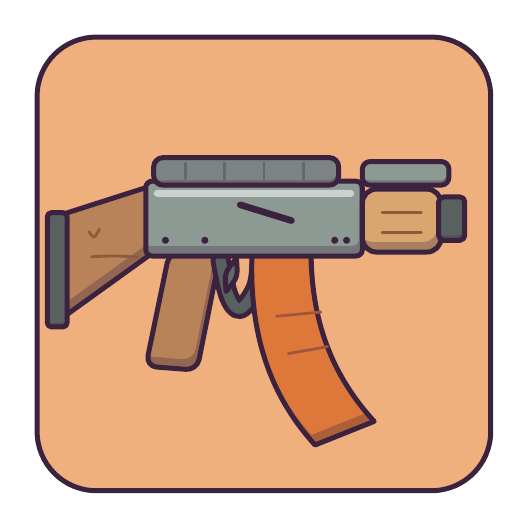
\begin{tikzpicture}
\clip (0,0) rectangle (6,6);
\fill[wallD] [rounded corners=0.75cm] (0.12,0.12) rectangle (5.88,5.88);
\begin{scope}\clip [rounded corners=0.75cm] (0.12,0.12) rectangle (5.88,5.88);
\begin{scope}\clip[rounded corners=0.08cm] (0.35,2.25) -- (1.6,3.15) -- (1.6,4) -- (0.35,3.6) -- cycle;
\fill[wood!70!ink,rounded corners=0.08cm] (0.35,2.25) -- (1.6,3.15) -- (1.6,4) -- (0.35,3.6) -- cycle;
\fill[wood,rounded corners=0.08cm, shift={(-0.045,0.13)}] (0.35,2.25) -- (1.6,3.15) -- (1.6,4) -- (0.35,3.6) -- cycle;
\end{scope}
\draw[inked,rounded corners=0.08cm] (0.35,2.25) -- (1.6,3.15) -- (1.6,4) -- (0.35,3.6) -- cycle;
\draw[wooddark, line width=1pt, line cap=round, line join=round] plot[smooth, tension=0.6] coordinates {(0.812,3.091) (1.102,3.1) (1.393,3.086)};
\draw[wooddark, line width=1pt, line cap=round, line join=round] plot[smooth, tension=0.6] coordinates {(0.778,3.409) (0.844,3.341) (0.91,3.443)};
\begin{scope}\clip[rounded corners=0.05cm] (0.25,2.2) rectangle (0.5,3.65);
\fill[metaldark!85!ink!70!ink,rounded corners=0.05cm] (0.25,2.2) rectangle (0.5,3.65);
\fill[metaldark!85!ink,rounded corners=0.05cm, shift={(-0.017,0.05)}] (0.25,2.2) rectangle (0.5,3.65);
\end{scope}
\draw[inked,rounded corners=0.05cm] (0.25,2.2) rectangle (0.5,3.65);
\begin{scope}\clip[rounded corners=0.14cm] (1.8,3.15) -- (2.45,3.15) -- (2.15,1.65) -- (1.5,1.7) -- cycle;
\fill[wood!70!ink,rounded corners=0.14cm] (1.8,3.15) -- (2.45,3.15) -- (2.15,1.65) -- (1.5,1.7) -- cycle;
\fill[wood,rounded corners=0.14cm, shift={(-0.045,0.13)}] (1.8,3.15) -- (2.45,3.15) -- (2.15,1.65) -- (1.5,1.7) -- cycle;
\end{scope}
\draw[inked,rounded corners=0.14cm] (1.8,3.15) -- (2.45,3.15) -- (2.15,1.65) -- (1.5,1.7) -- cycle;
\draw[ink, line width=7.299pt, line cap=round, line join=round] plot[smooth, tension=0.6] coordinates {(2.45,3.05) (2.55,2.6) (2.7,2.43) (2.9,2.7) (2.95,3.05)};
\draw[metaldark!85!ink, line width=3.699pt, line cap=round, line join=round] plot[smooth, tension=0.6] coordinates {(2.45,3.05) (2.55,2.6) (2.7,2.43) (2.9,2.7) (2.95,3.05)};
\filldraw[inked,fill=metaldark] (2.65,3.07) .. controls (2.671,2.833) .. (2.52,2.65) .. controls (2.499,2.887) .. (2.65,3.07) -- cycle;
\begin{scope}\clip (2.85,3.15) .. controls (2.8,2.0) and (3.15,1.25) .. (3.65,0.7) -- (4.4,1.0) .. controls (3.85,1.6) and (3.6,2.3) .. (3.6,3.15) -- cycle;
\fill[orange!80!wooddark!70!ink] (2.85,3.15) .. controls (2.8,2.0) and (3.15,1.25) .. (3.65,0.7) -- (4.4,1.0) .. controls (3.85,1.6) and (3.6,2.3) .. (3.6,3.15) -- cycle;
\fill[orange!80!wooddark, shift={(-0.045,0.13)}] (2.85,3.15) .. controls (2.8,2.0) and (3.15,1.25) .. (3.65,0.7) -- (4.4,1.0) .. controls (3.85,1.6) and (3.6,2.3) .. (3.6,3.15) -- cycle;
\end{scope}
\draw[inked] (2.85,3.15) .. controls (2.8,2.0) and (3.15,1.25) .. (3.65,0.7) -- (4.4,1.0) .. controls (3.85,1.6) and (3.6,2.3) .. (3.6,3.15) -- cycle;
\draw[orange!55!ink, line width=1.0pt, line cap=round] (3.16,2.335) -- (3.723,2.388);
\draw[orange!55!ink, line width=1.0pt, line cap=round] (3.31,1.86) -- (3.81,1.95);
\begin{scope}\clip[rounded corners=0.08cm] (1.5,3.1) rectangle (4.25,4.05);
\fill[metal!70!ink,rounded corners=0.08cm] (1.5,3.1) rectangle (4.25,4.05);
\fill[metal,rounded corners=0.08cm, shift={(-0.045,0.13)}] (1.5,3.1) rectangle (4.25,4.05);
\end{scope}
\draw[inked,rounded corners=0.08cm] (1.5,3.1) rectangle (4.25,4.05);
\begin{scope}\clip[rounded corners=0.12cm] (1.6,4) rectangle (3.95,4.35);
\fill[metal!80!ink!70!ink,rounded corners=0.12cm] (1.6,4) rectangle (3.95,4.35);
\fill[metal!80!ink,rounded corners=0.12cm, shift={(-0.021,0.06)}] (1.6,4) rectangle (3.95,4.35);
\end{scope}
\draw[inked,rounded corners=0.12cm] (1.6,4) rectangle (3.95,4.35);
\draw[metaldark, line width=1pt, line cap=round] (2,4.08) -- (2,4.28);
\draw[metaldark, line width=1pt, line cap=round] (2.5,4.08) -- (2.5,4.28);
\draw[metaldark, line width=1pt, line cap=round] (3,4.08) -- (3,4.28);
\draw[metaldark, line width=1pt, line cap=round] (3.5,4.08) -- (3.5,4.28);
\draw[ink, line width=2.4pt, line cap=round] (2.7,3.75) -- (3.35,3.55);
\fill[ink] (1.75,3.3) circle (0.045);
\fill[ink] (2.25,3.3) circle (0.045);
\fill[ink] (3.9,3.3) circle (0.045);
\fill[ink] (4.05,3.3) circle (0.045);
\fill[white, opacity=0.55, rounded corners=0.05cm] (1.6,3.85) rectangle (4.15,3.94);
\begin{scope}\clip[rounded corners=0.1cm] (4.25,4) rectangle (5.35,4.3);
\fill[metal!70!ink,rounded corners=0.1cm] (4.25,4) rectangle (5.35,4.3);
\fill[metal,rounded corners=0.1cm, shift={(-0.021,0.06)}] (4.25,4) rectangle (5.35,4.3);
\end{scope}
\draw[inked,rounded corners=0.1cm] (4.25,4) rectangle (5.35,4.3);
\begin{scope}\clip[rounded corners=0.18cm] (4.25,3.15) rectangle (5.25,3.95);
\fill[woodlight!70!ink,rounded corners=0.18cm] (4.25,3.15) rectangle (5.25,3.95);
\fill[woodlight,rounded corners=0.18cm, shift={(-0.045,0.13)}] (4.25,3.15) rectangle (5.25,3.95);
\end{scope}
\draw[inked,rounded corners=0.18cm] (4.25,3.15) rectangle (5.25,3.95);
\draw[wooddark, line width=1pt, line cap=round] (4.5,3.4) -- (5,3.4);
\draw[wooddark, line width=1pt, line cap=round] (4.5,3.65) -- (5,3.65);
\begin{scope}\clip[rounded corners=0.06cm] (5.22,3.3) rectangle (5.55,3.85);
\fill[metaldark!85!ink!70!ink,rounded corners=0.06cm] (5.22,3.3) rectangle (5.55,3.85);
\fill[metaldark!85!ink,rounded corners=0.06cm, shift={(-0.021,0.06)}] (5.22,3.3) rectangle (5.55,3.85);
\end{scope}
\draw[inked,rounded corners=0.06cm] (5.22,3.3) rectangle (5.55,3.85);
\end{scope}
\draw[inked] [rounded corners=0.75cm] (0.12,0.12) rectangle (5.88,5.88);
\end{tikzpicture}
\end{document}
